\documentclass{cslthse-msc}
\usepackage[utf8]{inputenc}
\usepackage[english]{babel}
\usepackage{amsmath}
\usepackage{amsfonts}
\usepackage{amssymb}
\usepackage{amsthm}
%\usepackage{makeidx}
\usepackage{graphicx}
\usepackage[titletoc, header, page]{appendix}
\usepackage{hyperref}

\usepackage{float}
\usepackage{listings}

%\geometry{showframe}

\author{
	Anton Fagerberg \\
	{\normalsize \href{mailto:ada10afa@student.lu.se}{\texttt{ada10afa@student.lu.se}}}
}

\title{Work in progress title}
\subtitle{A {\LaTeX} class}
\company{Jayway}
\supervisor{Roger Henriksson, \href{mailto:Roger.Henriksson@cs.lth.se}{\texttt{Roger.Henriksson@cs.lth.se}}}
\examiner{Görel Hedin, \href{mailto:Gorel.Hedin@cs.lth.se}{\texttt{Gorel.Hedin@cs.lth.se}}}

\date{\today}
%\date{February 18, 2014}

\acknowledgements{
If you want to thank people, do it here, on a separate right-hand page. Both the U.S. \textit{acknowledgments} and the British \textit{acknowledgements} spellings are acceptable.

We would like to thank Lennart Andersson for his feedback on this template.
}

\theabstract{
This document describes the Master's Thesis format for the theses carried out at 
the Department of Computer Science, Lund University. 

Your abstract should capture, in English, the whole thesis with focus on the problem and solution in 150 words. It should be placed on a separate right-hand page, with an additional \textit{1cm} margin on both left and right. Avoid acronyms, footnotes, and references in the abstract if possible.

Leave a \textit{2cm} vertical space after the abstract and provide a few keywords relevant for your report. Use five to six words, of which at most two should be from the title.
}

\keywords{MSc, template, report, style, structure}

%% Only used to display font sizes
\makeatletter
\newcommand\thefontsize[1]{{#1 \f@size pt\par}}
\makeatother
%%%%%%%%%%


\begin{document}
\makefrontmatter

\chapter{Performance issues with HTTP requests}

\section{Headers}

It is common in modern web applications to send a lot of HTTP requests. These requests can be very small, such as an GET request to update a field but the payload can also be considered very small when retrieving data from the server. Along with every HTTP request are plenty of headers. These headers can be a substantial part of every request and may therefore end up being the bottle neck if many small requests has to be performed.

As an example, consider the Instagram API\cite{instagram_api} which has an end-point where you can get information about a certain user account serialised in JSON format. If a client was built which is supposed to show details about, for example, the 10 most popular users, we can benchmark how making 10 separate API requests would differ from concatenating them into one request through an API-gateway.

\begin{figure}[H]
  \centering
    \begin{lstlisting}
{
    "data": {
        "id": "1574083",
        "username": "snoopdogg",
        "full_name": "Snoop Dogg",
        "profile_picture": "http://distillery...",
        "bio": "This is my bio",
        "website": "http://snoopdogg.com",
        "counts": {
            "media": 1320,
            "follows": 420,
            "followed_by": 3410
        }
    }
}
    \end{lstlisting}
  \caption{User data response from the Instagram API.}
\end{figure}

Performing HTTP requests can be benchmarked using cURL. To make the requests authentic, we tell cURL to use the default headers provided by the browser Firefox. These headers includes among other things browsers User-Agent, media types which are acceptable responses and so on.

\begin{figure}[H]
  \centering
\begin{lstlisting}[breaklines=true]
curl --trace-ascii - 'http://localhost:9000/user/snoopdogg' -H 'Host: localhost:9000' -H 'User-Agent: Mozilla/5.0 (Macintosh; Intel Mac OS X 10.10; rv:36.0) Gecko/20100101 Firefox/36.0' -H 'Accept: text/html,application/xhtml+xml,application/xml;q=0.9,*/*;q=0.8' -H 'Accept-Language: en-US,en;q=0.5' --compressed -H 'Connection: keep-alive' -H 'Pragma: no-cache' -H 'Cache-Control: no-cache'
\end{lstlisting}
  \caption{cURL command used in the benchmarks.}
\end{figure}

Performing this request will give us the following results:

\begin{figure}[H]
  \centering
\begin{lstlisting}[breaklines=true]
=> Send header, 355 bytes (0x163)
0000: GET /user/snoopdogg HTTP/1.1
001e: Accept-Encoding: deflate, gzip
003e: Host: localhost:9000
0054: User-Agent: Mozilla/5.0 (Macintosh; Intel Mac OS X 10.10; rv:36.
0094: 0) Gecko/20100101 Firefox/36.0
00b4: Accept: text/html,application/xhtml+xml,application/xml;q=0.9,*/
00f4: *;q=0.8
00fd: Accept-Language: en-US,en;q=0.5
011e: Connection: keep-alive
0136: Pragma: no-cache
0148: Cache-Control: no-cache
0161:
<= Recv header, 17 bytes (0x11)
0000: HTTP/1.1 200 OK
<= Recv header, 47 bytes (0x2f)
0000: Content-Type: application/json; charset=utf-8
<= Recv header, 21 bytes (0x15)
0000: Content-Length: 286
<= Recv header, 2 bytes (0x2)
0000:
<= Recv data, 286 bytes (0x11e)
\end{lstlisting}
  \caption{Results from cURL when performing a HTTP request to fetch one user. Actual payload omitted.}
\end{figure}

We can from this information see that 355 bytes are sent as header data, 87 bytes are then received as header data (17 + 47 + 21 + 2) and the actual payload is 286 bytes. This means 61\% of every request to this end-point are nothing but header data.

If we instead would expose an endpoint where all 10 users could be requested with one HTTP request which instead would return an array of JSON objects, we'll get the following result:

\begin{figure}[H]
  \centering
\begin{lstlisting}[breaklines=true]
=> Send header, 446 bytes (0x1be)
0000: GET /users/snoopdog1,snoopdog2,snoopdog3,snoopdog4,snoopdog5,sno
0040: opdog6,snoopdog7,snoopdog8,snoopdog9,snoopdo10 HTTP/1.1
0079: Accept-Encoding: deflate, gzip
0099: Host: localhost:9000
00af: User-Agent: Mozilla/5.0 (Macintosh; Intel Mac OS X 10.10; rv:36.
00ef: 0) Gecko/20100101 Firefox/36.0
010f: Accept: text/html,application/xhtml+xml,application/xml;q=0.9,*/
014f: *;q=0.8
0158: Accept-Language: en-US,en;q=0.5
0179: Connection: keep-alive
0191: Pragma: no-cache
01a3: Cache-Control: no-cache
01bc:
<= Recv header, 17 bytes (0x11)
0000: HTTP/1.1 200 OK
<= Recv header, 47 bytes (0x2f)
0000: Content-Type: application/json; charset=utf-8
<= Recv header, 22 bytes (0x16)
0000: Content-Length: 2871
<= Recv header, 2 bytes (0x2)
0000:
<= Recv data, 2871 bytes (0xb37)
\end{lstlisting}
  \caption{Results from cURL when performing a HTTP request to fetch 10 users. Actual payload omitted.}
\end{figure}

From the results, we can see that the sent headers are increased from 355 to 446 bytes because of the longer URL which specifies all users to fetch. The received headers are increased with just one byte from 87 to 88 because of the increased \emph{Content-Length} field. This results in a total header size of 534 bytes. The payload is increased from 286 bytes to 2871 bytes - about 10 fold as expected since we request 10 users at once instead of one at a time, the small increase is because of the array-characters in the JSON format. By avoiding doing 10 separate requests and instead do one concatenated request, the overhead from all headers have now been reduced from 61\% to 16\% and this will scale according to the number of requests - the more requests concatenated, the lesser amount of overhead from HTTP headers.

\begin{figure}[H]
  \centering
    \begin{center}
      \begin{tabular}{ r | c | c }
        \textbf{\#} & \textbf{10 users, 10 request} & \textbf{10 users, 1 request} \\ \hline
        Headers & 4,420 B & 534 B \\ \hline
        Payload & 2,860 B & 2,871 B \\ \hline
        \% headers of total data & 61\% & 16\% \\ \hline
      \end{tabular}
    \end{center}
  \caption{Header and payload ratio when doing 10 separate or one concatenated request to fetch users.}
\end{figure}

The data displayed in this example should be viewed as a lower bound. In practise, HTTP cookies which are used for personalisation, analytics and session management are also sent with every HTTP request an can add up to multiple kilobytes of protocol overhead for every HTTP request\cite[p. 200]{HPBN}.

This is one of the issues that may be mitigated by using HTTPS/2.0 which knows which headers that has already been sent and therefore doesn't need to retransmit them on subsequent requests\cite[p. 222]{HPBN}.

\section{Maximum TCP connections}
The HTTP 1.X protocol doesn't allow data to be multiplexed over the same connection\cite[p.194]{HPBN}. For this reason, browser vendors has introduced a connection pool of ~6 TCP connections per host (the HTTP 1.1 specification limits it to 2 connections\cite{rfc2616}, but modern browsers has refused to conform to this).

A common way to deal with this issue is domain sharding. Since the limit of 6 TCP connections are on a host basis, it is possible to create multiple subdomains to mitigate this problem. If the subdomains \{shard1, shard2, \ldots\}.example.com was created and pointed to the same server, more than 6 TCP connections can be used in parallel at the same time from that machine. This approach is not without downsides as every new host requires a new DNS lookup, a TCP 3-Way handshake and a TCP slow start from TCP which can slow down the user experience\cite[p. 199]{HPBN} - just the DNS lookup typically takes 20-120 ms\cite[p. 63]{HPWS}. - just the DNS The browser always opens 6 connections per shard automatically even if not all of them are used. Sharding can be a complicated manual process and it is hard to decide how many shards to use for optimal performance.

As an example, we can look at downloading thumbnails for an image gallery. Suppose we want to download 60 base64-encoded thumbnails and the connection we are using has a lot of bandwidth but high latency.

If all images were downloaded by using a single HTTP request per thumbnail, we can clearly see that the 6 TCP connection limit will become the bottleneck.

\begin{figure}[H]
  \centering
    \begin{center}
      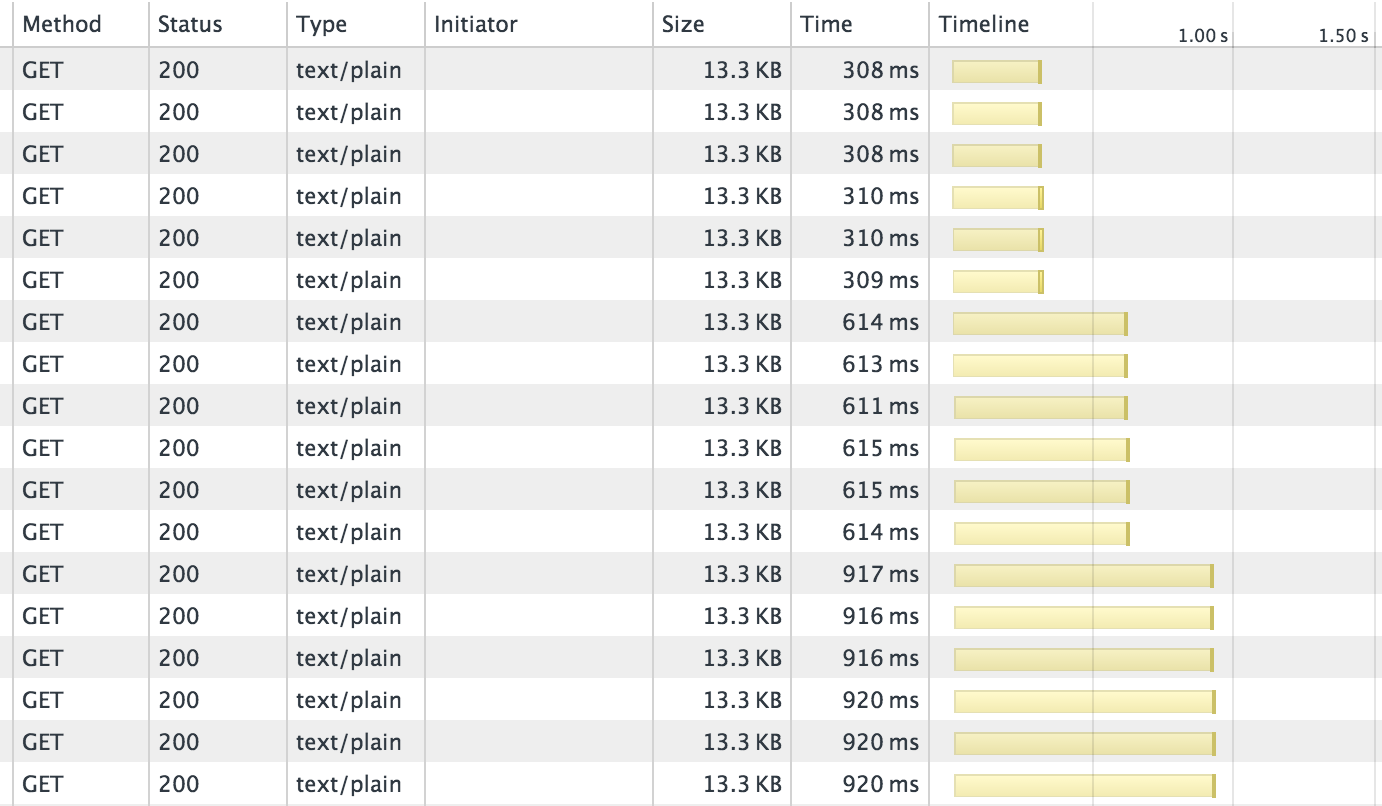
\includegraphics[width=0.9\textwidth]{images/chrome_latency_limit.png}
    \end{center}
  \caption{Chrome developer tools showing how the 6 TCP connection limit becomes a bottle neck on a connection with ~300 ms of latency.}
\end{figure}

We can calculate the total delay caused by latency in our example by this formula:

\begin{equation}
\mbox{total latency} = \mbox{number of thumbnails} * \frac{\mbox{latency per request}}{\mbox{nr of parallel requests}}
\end{equation}

In our example, we fetch 60 thumbnails and with a latency of ~300 ms per request. Our browser can handle 6 parallel connections which gives us the following result:

\begin{equation}
\mbox{total latency} = 60 * \frac{300}{6} = 3,000 \mbox{ ms}
\end{equation}

If we instead could concatenate these 60 thumbnail requests into one request to an API-gateway which in turn would fetch the 60 thumbnails and respond with all of them at once - then we would only have to pay the latency cost once which would reduce the total latency from 3,000 ms to 300 ms.

It is worth pointing out that increasing bandwidth would not resolve this problem as the latency is the only bottleneck in this scenario. It is not uncommon for browsers to wait 100 - 150 ms before spending 5 ms to download an image which means that latency is accounting for 90-95\% of the total time for the HTTP request\cite{latency}.

\subsection{Chunked responses}
When fetching thumbnails, you often want to display them as soon as each individual image is loaded and not wait for all of them to load before displaying them. When using a concatenated request to fetch all of them at the same time, the server can use chunked transfer encoding in the HTTP response to send the thumbnail data in chunks\cite{chunked}. By doing so, images can be loaded as soon as they are available, even out of order. This technique has been implemented by Dropbox as their solution for improved performance when displaying thumbnails\cite{dropbox_chunked}.

\section{Compression}

An API-gateway can compress the requested data before it is sent to the client. A common compression algorithm is Gzip (GNU Zip) which works best on text-based files, such as HTML, CSS and JavaScript. Gzip has an expected compression rate of 60-80\% when used on text-based files\cite[p. 237]{HPBN}.

It is worth mentioning that there are scenarios where Gzip compression applied to very small files can increase the total size because of the Gzip dictionary overhead\cite{google_gzip}.


As an example, user data for 50 users was created and stored in JSON format. When this was requested from the server without compression, the total content-length of the HTTP request payload was 55,205 bytes. When tunnelling this request through the API-gateway which compresses this data using Gzip, the content length was reduced to 16,563, which amounts to a space saving of 70\%. 

\begin{equation}
\mbox{Space Saving} = 1 - \frac{\mbox{Compressed Size}}{\mbox{Uncompressed Size}} = 1 - \frac{16,563}{55,205} = 70\%
\end{equation}

An important thing to note about Gzip compression is that only the payload is compressed in HTTP 1.1\cite{header_compression}. This means that the headers including cookies are not compressed which would've otherwise been an additional performance gain. This is one of the improvements which have been addressed in HTTP/2\cite[p. 222]{HPBN}.

\makebibliography{anton_msc}

\end{document}